\documentclass{article}

\usepackage{amsmath,amsfonts}
\usepackage{geometry}
\usepackage{graphicx}
\usepackage{xcolor}

\title{PVI Memory Safety}

\begin{document}

\newcommand{\tagcolor}{C}

\newcommand{\vt}{\mathit{vt}}
\newcommand{\pt}{\mathit{pt}}
\newcommand{\lt}{\mathit{lt}}
\newcommand{\lts}{\overline{\lt}}
\newcommand{\nt}{\mathit{nt}}
\newcommand{\PCT}{\mathcal{P}}

\newcommand{\trule}[2]{#1 \leftarrow #2}

\newcommand{\truledef}[1]{
  & \multispan{3} \(#1\) \\}

\newcommand{\assert}[1]{& & & \multispan{2} \(\mathbf{assert} ~ #1\) \hfill \\}
\newcommand{\letin}[1]{& & & \multispan{2} \(\mathit{let} ~ #1 ~ \mathit{in}\) \\}

\newcommand{\caseof}[1]{\textnormal{case } #1 \textnormal{ of}}
\newcommand{\caseentry}[2]{& & & #1 \Rightarrow #2}

\newcommand{\optional}[1]{\fcolorbox{black}{gray!20}{#1}}
\newcommand{\settag}[2]{\boldsymbol{#1} & \longleftarrow & & \mathit{#2}\\}
\newcommand{\settagopt}[2]{\optional{\(\boldsymbol{#1}\)} & \longleftarrow & & \mathit{#2}\\}

%%% Tag Rules %%%
\newcommand{\loadtname}{\mathbf{LoadT}}
\newcommand{\loadtargs}{\PCT, \pt, \vt, \overline{\lt}}
\newcommand{\loadtres}{\vt'}
\newcommand{\loadt}{\loadtname(\loadtargs)}

\newcommand{\storetname}{\mathbf{StoreT}}
\newcommand{\storetargs}{\PCT, \pt, \vt_1, \vt_2, \overline{\lt}}
\newcommand{\storetres}{\PCT',\vt',\overline{\lt}'}
\newcommand{\storet}{\storetname(\storetargs)}

\newcommand{\consttname}{\mathbf{ConstT}}
\newcommand{\consttres}{\vt}
\newcommand{\constt}{\consttname}

\newcommand{\unoptname}{\mathbf{UnopT}}
\newcommand{\unoptargs}{\PCT, \vt}
\newcommand{\unoptres}{\vt}
\newcommand{\unopt}{\unoptname(\unoptargs)}

\newcommand{\binoptname}{\mathbf{BinopT}}
\newcommand{\binoptargs}{\PCT, \vt_1, \vt_2}
\newcommand{\binoptres}{\vt'}
\newcommand{\binopt}{\binoptname(\binoptargs)}

\newcommand{\globaltname}{\mathbf{GlobalT}}
\newcommand{\globaltargs}{id, s}
\newcommand{\globaltargstyped}{id \in ident, s \in \mathbb{N}}
\newcommand{\globaltres}{\pt,\vt,\overline{\lt}}
\newcommand{\globalt}{\globaltname(\globaltargs)}

\newcommand{\localtname}{\mathbf{LocalT}}
\newcommand{\localtargs}{\PCT, id, s}
\newcommand{\localtargstyped}{\PCT, id \in ident, s \in \mathbb{N}}
\newcommand{\localtres}{\pt,\vt,\overline{\lt}}
\newcommand{\localt}{\localtname(\localtargs)}

\newcommand{\vartname}{\mathbf{VarT}}
\newcommand{\vartargs}{\PCT, \vt}
\newcommand{\vartres}{\pt}
\newcommand{\vart}{\vartname(\vartargs)}

\newcommand{\malloctname}{\mathbf{MallocT}}
\newcommand{\malloctargs}{\PCT, \vt}
\newcommand{\malloctres}{\PCT',\pt,\optional{\(\vt,\overline{\lt}\)}}
\newcommand{\malloct}{\malloctname(\malloctargs)}

\newcommand{\freetname}{\mathbf{FreeT}}
\newcommand{\freetargs}{\PCT, \vt}
\newcommand{\freetres}{\PCT',\pt,\optional{\(\vt,\overline{\lt}\)}}
\newcommand{\freet}{\freetname(\freetargs)}

\newcommand{\picasttname}{\mathbf{PICastT}}
\newcommand{\picasttargs}{\PCT, \pt, \optional{\(\vt, \overline{\lt}\)}}
\newcommand{\picasttres}{\PCT',\vt}
\newcommand{\picastt}{\picasttname(\picasttargs)}

\newcommand{\ipcasttname}{\mathbf{IPCastT}}
\newcommand{\ipcasttargs}{\PCT, \vt_1, \optional{\(\vt_2, \overline{\lt}\)}}
\newcommand{\ipcasttres}{\PCT',\pt}
\newcommand{\ipcastt}{\ipcasttname(\ipcasttargs)}

\newcommand{\ppcasttname}{\mathbf{PPCastT}}
\newcommand{\ppcasttargs}{\PCT, \pt, \optional{\(\vt, \overline{\lt}\)}}
\newcommand{\ppcasttres}{\PCT',\pt'}
\newcommand{\ppcastt}{\picasttname(\picasttargs)}

\newcommand{\iicasttname}{\mathbf{IICastT}}
\newcommand{\iicasttargs}{\PCT, \vt_1}
\newcommand{\iicasttres}{\PCT',\pt}
\newcommand{\iicastt}{\ipcasttname(\ipcasttargs)}

\newcommand{\splittname}{\mathbf{SplitT}}
\newcommand{\splittargs}{\PCT, \vt, \optional{\(L\)}}
\newcommand{\splittres}{\PCT'}
\newcommand{\splitt}{\splittname(\splittargs)}
           
\newcommand{\jointname}{\mathbf{JointT}}
\newcommand{\jointargs}{\PCT, \optional{\(L\)}}
\newcommand{\jointres}{\PCT'}
\newcommand{\joint}{\jointname(\jointargs)}

\newcommand{\argtname}{\mathbf{ArgT}}
\newcommand{\argtargs}{\PCT, \vt, f, x}
\newcommand{\argtargstyped}{\PCT, \vt, f, x \in ident}
\newcommand{\argtres}{\vt'}
\newcommand{\argt}{\argtname(\argtargs)}

\newcommand{\callerrettname}{\mathbf{CallerRetT}}
\newcommand{\callerrettargs}{\PCT, \PCT', \vt}
\newcommand{\callerrettres}{\vt'}
\newcommand{\callerrett}{\callerrettname(\callerrettargs)}

\newcommand{\calleerettname}{\mathbf{CalleeRetT}}
\newcommand{\calleerettargs}{\PCT, \PCT', \vt}
\newcommand{\calleerettres}{\vt'}
\newcommand{\calleerett}{\calleerettname(\calleerettargs)}

%%%%%%%%%%%%%%%%%

%%% Continuations, States, Values %%%

\newcommand{\kemp}{\mathit{Kemp}}
\newcommand{\kdo}[1]{\mathit{Kdo};~ #1}
\newcommand{\kseq}[2]{\mathit{Kseq} ~ #1; ~ #2}
\newcommand{\kif}[4]{\mathit{Kif}[#1 \mid #2] ~ \mathit{join} ~ #3; ~ #4}
\newcommand{\kwhiletest}[4]{\mathit{KwhileTest}(#1) ~ \{ ~ #2 ~ \} ~ \mathit{join} ~ #3; ~ #4}
\newcommand{\kwhileloop}[4]{\mathit{KwhileLoop}(#1) ~ \{ ~ #2 ~ \} ~ \mathit{join} ~ #3; ~ #4}
\newcommand{\kdowhiletest}[4]{\mathit{KdoWhileTest}(#1) ~ \{ ~ #2 ~ \} ~ \mathit{join} ~ #3; ~ #4}
\newcommand{\kdowhileloop}[4]{\mathit{KdoWhileLoop}(#1) ~ \{ ~ #2 ~ \} ~ \mathit{join} ~ #3; ~ #4}
\newcommand{\kfor}[2]{\mathit{Kfor} ~ #1; ~ #2}
\newcommand{\kforpost}[2]{\mathit{KforPost} ~ #1; ~ #2}
\newcommand{\kcall}[3]{\mathit{Kcall} ~ #1 ~ #2 ~ #3}

\newcommand{\ctx}[1]{ctx \left[#1\right]}

\newcommand{\sstate}[6]{\mathcal{S}\left(f,#2,#3,#4 \mid #5 \gg #6 @ #1\right)}
\newcommand{\estate}[6]{\mathcal{E}\left(f,#2,#3,#4 \mid #5; \gg #6 @ #1\right)}
\newcommand{\cstate}[7]{\mathcal{C}\left(#1,#3,#4 \mid #5(#6) \gg #7 @ #2\right)}
\newcommand{\rstate}[6]{\mathcal{R}\left(#1,#3,#4 \mid #5 \gg #6 @ #2\right)}
\newcommand{\fstate}[1]{\mathcal{F}\left(#1\right)}

\newcommand{\mem}{m}
\newcommand{\genv}{\mathit{ge}}
\newcommand{\lenv}{\mathit{le}}
\newcommand{\cont}{k}
\newcommand{\stmt}{s}
\newcommand{\expr}{e}
\newcommand{\type}{ty}
\newcommand{\defestate}[1]
           {\estate{\PCT}{\mem}{\genv}{\lenv}{#1}{\cont}}
\newcommand{\defsstate}[1]
           {\sstate{\PCT}{\mem}{\genv}{\lenv}{#1}{\cont}}

\newcommand{\valof}[1]{|#1|}
\newcommand{\deref}[1]{* #1}
\newcommand{\addrof}[1]{\& #1}
\newcommand{\assignop}[3]{#2 ~~ [#1]\!\!= #3}
\newcommand{\postinc}[2]{#2 #1\!\!#1}
\newcommand{\assign}[2]{#1 := #2}
\newcommand{\loc}[2]{\underline{#1}@#2}
\newcommand{\val}[2]{\mathit{#1} @ #2}
\newcommand{\binop}[3]{#2 #1 #3}
\newcommand{\unop}[2]{#1 #2}
\newcommand{\comma}[2]{#1, #2}
\newcommand{\paren}[2]{(#2) (#1)}
\newcommand{\builtin}[2]{\mathit{builtin} ~ #1(#2)}
\newcommand{\var}[1]{#1}
\newcommand{\cast}[2]{(#2) #1}
\newcommand{\call}[2]{#1(#2)}
\newcommand{\condition}[3]{#1 ~ ? ~ #2 ~ : ~ #3}
\newcommand{\sizeof}[1]{\mathtt{size}(#1)}
\newcommand{\alignof}[1]{\mathtt{align}(#1)}

\newcommand{\sskip}{\mathtt{skip}}
\newcommand{\sdo}[1]{#1;}
\newcommand{\sseq}[2]{#1 ~ #2}
\newcommand{\scontinue}{\mathtt{continue}}
\newcommand{\sbreak}{\mathtt{break}}
\newcommand{\sreturn}{\mathtt{return}}
\newcommand{\sifthenelse}[4]{\mathtt{if}(#1) ~ \mathtt{then} ~ #2 ~ \mathtt{else} ~ #3 ~ \mathtt{join} ~ #4}
\newcommand{\swhile}[3]{\mathtt{while}(#1) ~ \mathtt{do} ~ #2 ~ \mathtt{join} ~ #3}
\newcommand{\sdowhile}[3]{\mathtt{do} ~ #2 ~ \mathtt{while} ~ (#1) ~ \mathtt{join} ~ #3}
\newcommand{\sfor}[5]{\mathtt{for}(#1; #2; #3) ~ \mathtt{do} ~ #4 ~ \mathtt{join} ~ #5}
\newcommand{\sswitch}[2]{\mathtt{switch} ~ #1 ~ \{ ~ #2 ~ \}}
\newcommand{\slabel}[2]{#1: ~ #2}
\newcommand{\sgoto}[1]{\mathtt{goto} ~ #1}

\newcommand{\vundef}{\mathbf{undef}}

\newcommand{\tptr}[1]{\mathit{ptr(#1)}}

\newcommand{\judgment}[3][]{
  {\centering
  \smallskip
  \begin{tabular}{c}
    #2 \\
    \hline
    #3
  \end{tabular}{\sc #1}
  \smallskip\par}}

\newcommand{\judgmentbr}[4][]{
  {\centering
  \smallskip
  \begin{tabular}{c}
    #2 \\
    #3 \\
    \hline
    #4
  \end{tabular}{\sc #1}
   \smallskip\par}}

\newcommand{\judgmentbrbr}[5][]{
  {\centering
  \smallskip
  \begin{tabular}{c}
    #2 \\
    #3 \\
    #4 \\
    \hline
    #5
  \end{tabular}{\sc #1}
   \smallskip\par}}

\newcommand{\judgmentbrbrbr}[6][]{
  {\centering
  \smallskip
  \begin{tabular}{c}
    #2 \\
    #3 \\
    #4 \\
    #5 \\
    \hline
    #6
  \end{tabular}{\sc #1}
   \smallskip\par}}

\newcommand{\judgmenttwobr}[6][]{
  {
    \centering
    \smallskip
    \begin{tabular}{c c}
       #2 & #3 \\
       #4 & #5 \\
       \hline
       \multicolumn{2}{c}{#6}
    \end{tabular}{\sc #1}
    \vspace{\belowdisplayskip}\par
  }}

\newcommand{\judgmenttwobrlong}[5][]{
  {
    \centering
    \smallskip
    \begin{tabular}{c c}
       #2 & #3 \\
       \multicolumn{2}{c}{#4} \\
       \hline
       \multicolumn{2}{c}{#5}
    \end{tabular}{\sc #1}
    \vspace{\belowdisplayskip}\par
  }}

\newcommand{\judgmentthreebrlong}[6][]{
  {
    \centering
    \smallskip
    \begin{tabular}{c c c}
       #2 & #3 & #4 \\
       \multicolumn{3}{c}{#5} \\
       \hline
       \multicolumn{3}{c}{#6}
    \end{tabular}{\sc #1}
    \vspace{\belowdisplayskip}\par
  }}

\newcommand{\judgmentthreebrtwo}[7][]{
  {
    \centering
    \smallskip
    \begin{tabular}{c c c}
       #2 & #3 & #4 \\
       \multicolumn{3}{c}{#5 \hfill #6} \\
       \hline
       \multicolumn{3}{c}{#7}
    \end{tabular}{\sc #1}
    \vspace{\belowdisplayskip}\par
  }}

\newcommand{\judgmenttwobrlongbrlong}[6][]{
  {
    \centering
    \smallskip
    \begin{tabular}{c c}
       #2 & #3 \\
       \multicolumn{2}{c}{#4} \\
       \multicolumn{2}{c}{#5} \\
       \hline
       \multicolumn{2}{c}{#6} \\
    \end{tabular}{\sc #1}
    \vspace{\belowdisplayskip}\par
  }}


\newcommand{\judgmentthreebr}[8][]{
  {
    \centering
    \smallskip
    \begin{tabular}{c c c}
       #2 & #3 & #4 \\
       #5 & #6 & #7 \\
       \hline
       \multicolumn{3}{c}{#8}
    \end{tabular}{\sc #1}
    \vspace{\belowdisplayskip}\par
  }}


\newcommand{\judgmenttwo}[4][]{
  {\centering
  \smallskip
  \begin{tabular}{c c}
    #2 & #3 \\
    \hline
    \multicolumn{2}{c}{#4}
  \end{tabular}{\sc #1}
  \smallskip\par}}

\newcommand{\judgmentthree}[5][]{
  {\centering
  \smallskip
  \begin{tabular}{c c c}
    #2 & #3 & #4 \\
    \hline
    \multicolumn{3}{c}{#5}
  \end{tabular}{\sc #1}
  \smallskip\par}}

\newcommand{\judgmentfour}[6][]{
  {\centering
  \smallskip
  \begin{tabular}{c c c c}
    #2 & #3 & #4 & #5 \\
    \hline
    \multicolumn{4}{c}{#6}
  \end{tabular}{\sc #1}
  \smallskip\par}}


\section{Assumptions}

This write-up presents my PVI and PNVI memory safety policies. In the interest of being able
to slot it into the eventual paper and thesis, I'm assuming that the semantics have already
been presented at a high level, along with the standard explanations of what tags and control
points are.

One thing that needs to be called out is the way that tags work on memory. A memory is an
array of bytes, and a load or store will access some number of bytes. I write
\(\mem[l]_s = v@\vt @\overline{\lt}\) to denote loading \(s\) bytes,
starting at location \(l\), and interpreting them as a value \(v\), a value tag \(\vt\), and a list of
\(s\) location tags. Likewise, \(\mem[l \mapsto v@\vt @ \overline{lt}]_s\)
denotes storing that many bytes. Note the distinction between \(\vt\) and \(\overline{lt}\).
The former is tied to each full value, which may consist of multiple bytes, while the latter is tied
to an individual byte. When writing multiple contiguous values, I will write a range of locations. So
in the case of an array of 10 integers, \(s\) would be 4, and
\(\mem[l \dots l+10 \mapsto v@\vt @ \overline{lt}]_4\) would write \(v@\vt\) to ten words starting at \(l\),
with the four bytes of each word tagged with \(\overline{lt}\)'s four tags.
This guarantees that even misaligned loads and stores always have a valid location tag to check
(possibly multiple, mismatched location tags, in which case the policy can failstop if needed.)

\paragraph*{Control Points with Side-effects and Optional Arguments}

Most control points can be mapped cleanly onto one or more instructions in a compiled
program. For example, the \(\mathbf{BinopT}\) control point takes as input the tags on the parameters
of an operation (as well as the PC tag) and yields a tag for the result, so the target-level
rule, which does the same, can be identical. Other control points may correspond to multiple
target-level instructions, requiring a more complicated mapping. I will not call these out
unless they are particularly noteworthy. From a performance standpoint, the most problematic
situation is when a Tagged-C control point requires a tag from a location that is not read under
a normal compilation scheme, which must update tags in locations that are not written, or in which
the source construct does not have corresponding instructions in the targetl.

These situations require the compiler to add instructions for the primary purpose of manipulating
tags. If the tag rules that instantiate those control points do not make use of them, these instructions
are needless overhead. In these cases, the control points will take optional parameters or return
optional results, and I will explain how the rule should be implemented in the target if the
options are used. If compiling with a known policy that does not make use of the options, it will
be sound to eliminate the extra instructions. If {\it all} of the control point's outputs are
optional and unused, the control point need not be compiled at all. In this document, optional inputs
and outputs will be marked with \(\optional{boxes}\).

\section{Memory safety basics}

Memory safety policies operate on under a ``lock and key'' model, in which objects in memory
are tagged with a unique identifier (the ``lock'') and may only be accessed via a pointer tagged
with the same identifier (the ``key.'') For a simple example, consider the following code:
%
\vspace{\abovedisplayskip}
\begin{verbatim}
void main() {
  int a[10];
  int b[10];
  a[10] = 42;    
}
\end{verbatim}
\vspace{\belowdisplayskip}
%
In a typical stack allocator---such as the one used by my interpreter---{\tt a} and {\tt b} will
be allocated next to one another on the stack, like this:

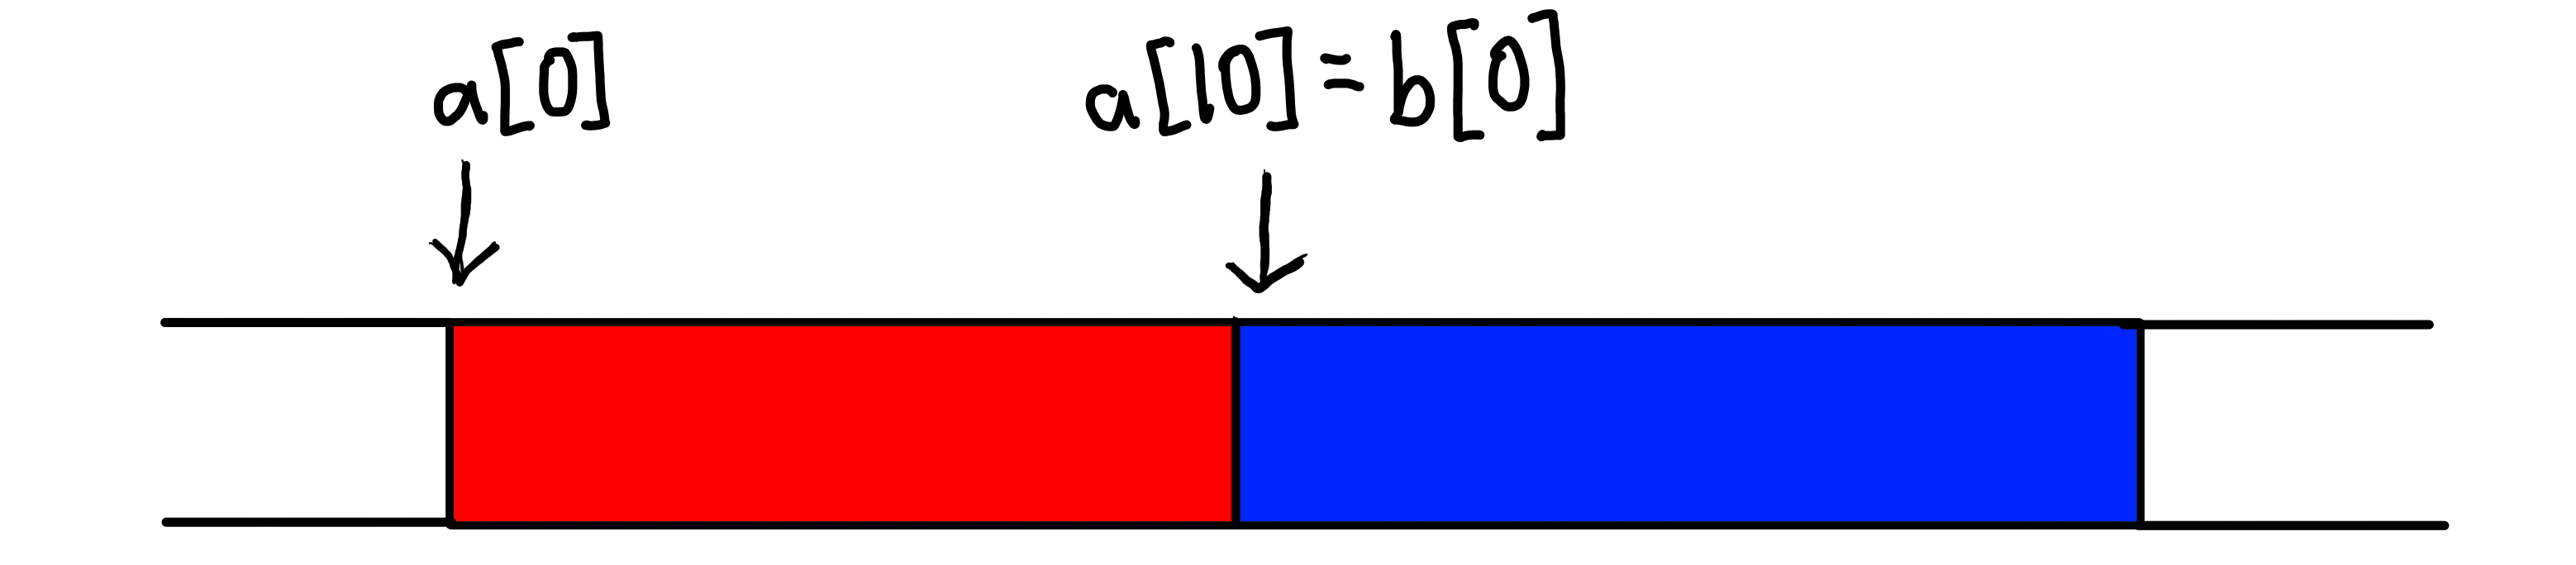
\includegraphics[width=.5\textwidth]{example.png}

To prevent the expression {\tt a[10] = 42} from overwriting {\tt b[0]}, we give {\tt a} and {\tt b}
unique {\it color tags} when they are allocated. In this case, we'll tag {\tt a} with \(\mathit{dyn ~ 0}\),
indicating that it's the first dynamically allocated object, and {\tt b} with \(\mathit{dyn ~ 1}\).
Then, when we evaluate the left-hand expression {\tt a} into its memory location \(l\), we tag
\(l\) with \(\mathit{dyn ~ 0}\). When we take the offset \(l + 10\), we keep that tag. And when we
perform the assignment, we check that the location tag at \(l\) matches. It doesn't, so we failstop.

The same principle applies for this code:

\vspace{\abovedisplayskip}
\begin{verbatim}
void main() {
  int* a = malloc(10 * sizeof(int));
  int* b = malloc(10 * sizeof(int));
  *(a + (b - a)) = 42;
}
\end{verbatim}
\vspace{\belowdisplayskip}

In this case, {\tt a} and {\tt b} could be allocated anywhere in the heap, and in Tagged C
the expression {\tt *(a + (b - a)) = 42} will always write to {\tt *b}. While this might be intentional
on the part of the programmer, it is also undefined behavior in the C standard, and in some
(but not all; see below) formal C semantics. Likewise, if {\tt a} and {\tt b} are next to each other
or in some other predictable arrangement, arithmetic like our first example can apply.
The memory safety policy works just the same in this scenario, with the tags being attached
by the call to malloc, once again using the \(\mathit{dyn}\) label in a global count of allocated blocks.
Meanwhile, values that are not derived from valid pointers at all are tagged \(X\), and can never
be read or written through, to avoid pointer forging, like this:

\vspace{\abovedisplayskip}
\begin{verbatim}
void main() {
  int* a = malloc(10 * sizeof(int));
  // I happen to know that a will be at address 1000
  *1000 = 42;
}
\end{verbatim}
\vspace{\belowdisplayskip}

Both stack and heap allocations use the \(\mathit{dyn}\) label and have a color that can grow arbitrarily
high. This is because over a program's execution, it might allocate an unbounded number of heap- or
stack-allocated objects, and each needs a unique identifier. Existing work has shown that in practice,
tag colors can be ``garbage collected'' and reused, but in Tagged C we assume them to be infinite and unique.

Lastly, we have global variables. While ``global safety'' is not as prominent a topic as heap or
stack safety, overrunning a global buffer is still a problem. It is also easy to forge a pointer to a global,
and when this happens it can undermine assumptions about the behavior of linked libraries whose globals
are not exported. Globals do not need dynamic colors, but can use their identifiers as tags, of the form
\(\mathit{glob} ~ id\).

\section{PVI and PNVI}

Our policies aim to enforce two memory models in particular: {\it PVI} (provenanace via integer) and
{\it PNVI} (provenance not via integer) from Memarian et al. \cite{???}. They propose PVI and PNVI
as memory models that support common idioms that are undefined in the C standard, but are still restrictive
enough as to support useful alias analysis for optimization. This application is orthogonal to
security, and violations of either memory model are treated as undefined behavior, just as in the
C standard. Our goal is to turn that UB into failstop behavior, so that undefined programs cannot accidentally
undermine their own security.

Both memory models represent pointers as integers, just as Tagged C does, with additional provenance
associated with each object. An integer cast to a pointer in PVI retains this provenance, enabling
integer operations to be performed on it prior to it being cast back to a pointer.
In PNVI, by contrast, an integer cast to a pointer gains the provenance of the object it points
to when the cast occurs. While PNVI supports a wider range of programs, it is inconsistent with important
assumptions of the C memory model, in ways that may have serious security consequences.
The difference between PVI and PNVI is illustrated in Figure \ref{fig:PVI-PNVI}.

\begin{figure}
  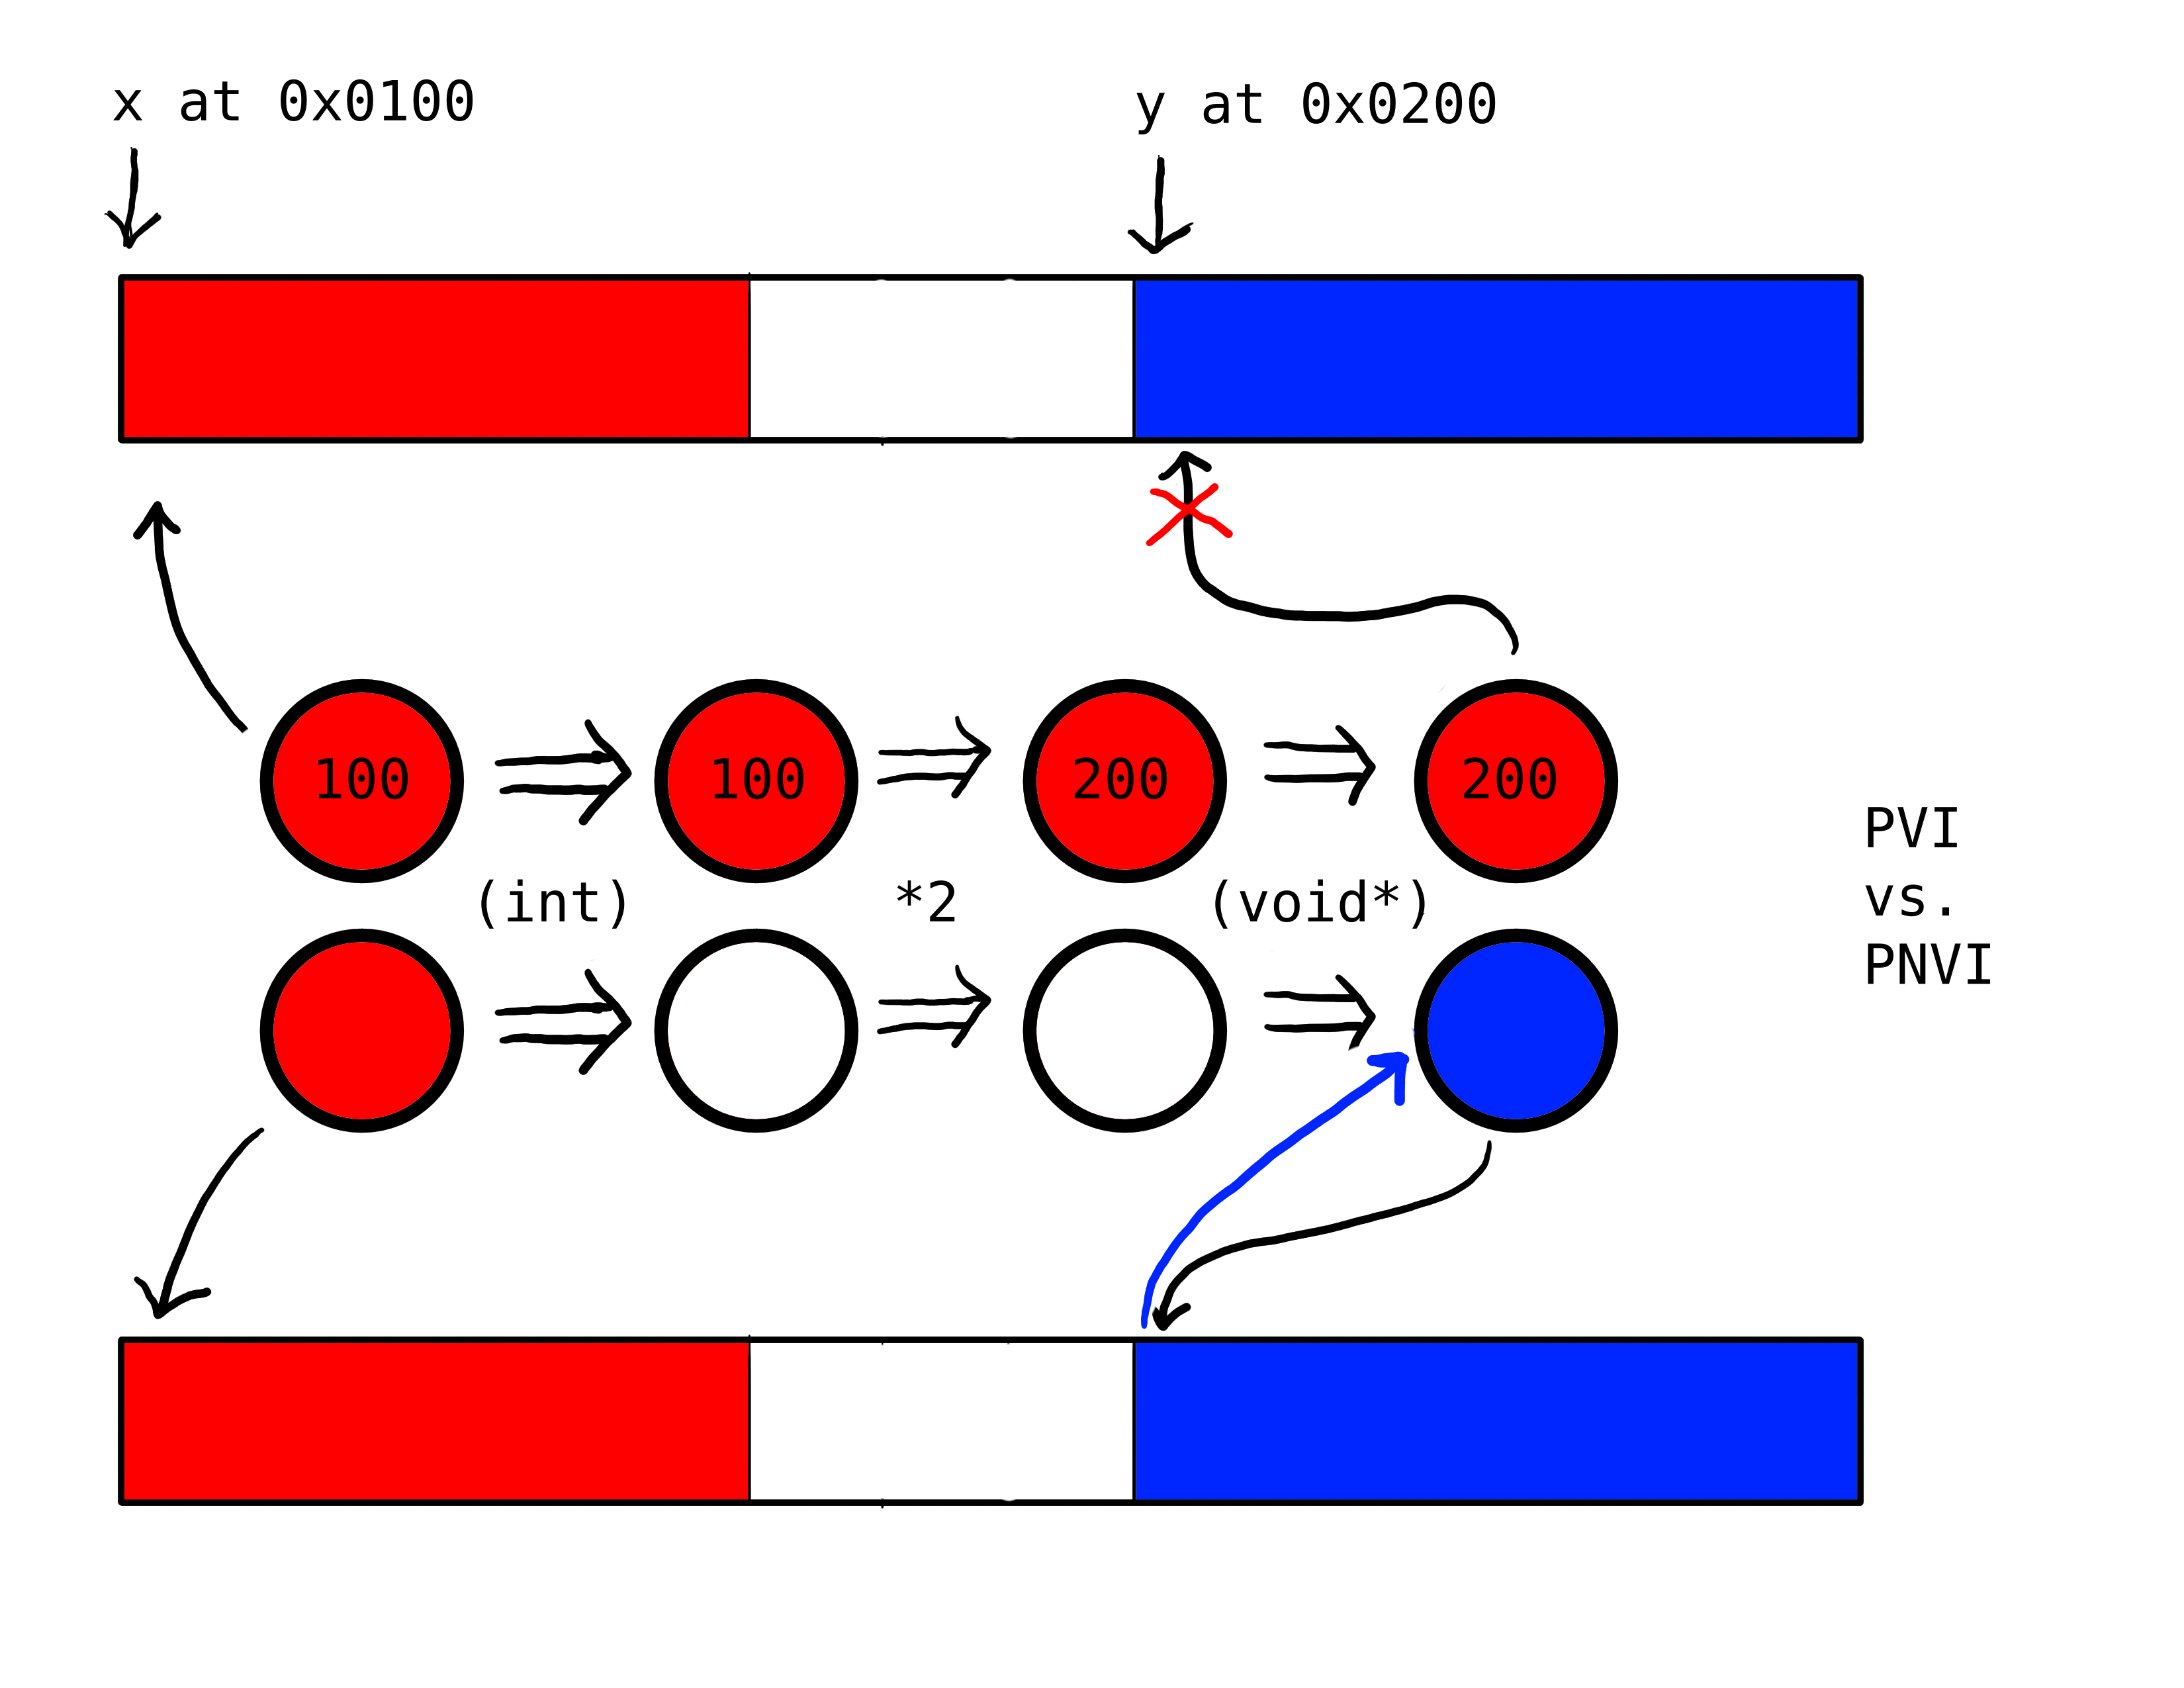
\includegraphics[width=.6\textwidth]{PVIvsPNVI.png}
  \caption{Integer-pointer casts in PVI and PNVI}
  \label{fig:PVI-PNVI}
\end{figure}

We will aim to prove that for any program, if it is run in both the PVI semantics
and in Tagged C with our PVI policy, it either produces identical output, or it is both
undefined in the PVI semantics and failstops in Tagged C. Likewise for PNVI, except that
some UB in PNVI is non-deterministic, and we only require that it failstop in an execution
that would {\it reach} the UB.

\section{PVI Definitions}

Here we give the relevant tag rules for the PVI policy, and describe the control points that
they attach to. We will, for each rule, first give the control point(s) that use it, along
with a brief explanation of what the surrounding semantics rules do, and then give the rule.
For these policies, all control points appear in expression reduction steps.
The machine state consists of the PC tag \(\PCT\), a memory \(\mem\),
the global environment \(\genv\), and a local environment \(\lenv\). These are contextual semantics,
so each expression is situated in some context \(\mathit{ctx}\).

The core of the PVI policy is the {\it provenance color}, represented
by a natural number.
%
\begin{align*}
  T ::= & \mathit{glob} ~ id & id \in \mathit{ident} \\
  & \mathit{dyn} ~ \tagcolor & \tagcolor \in \mathbb{N} \\
\end{align*}

\paragraph*{Color generation}

New colors are generated when objects are allocated. When exactly that occurs
depends on where the object lives. Global variables are a special case: they are
allocated during program initialization, before execution begins. As such they
do not have a control point per se, but a rule that functions similarly, while
being more expressive.

%All of our allocation control points differ from the normal ones in that they
%pass a type as a parameter and recieve a list of tags that they apply to
%a memory region of the size of that type.

Given a list \(xs\) of variable identifiers \(id\) and types
\(ty\), a program's initial memory is defined by iteratively allocating each one
in memory and updating the global environment with its base address, bound, type,
and a static identity tag. Let \(|ty|\) be a function from types to their sizes
in bytes. The memory is initialized \(\vundef@\vt@\overline{\lt}\)
for some \(\vt\) and \(\overline{\lt}\), unless given an initializer.
Let \(\mem_0\) and \(\genv_0\) be the initial (empty) memory and environment.
The parameter \(b\) marks the start of the global region.

%Since we don't need to initialize tags in memory dynamically, our rule for
%selecting these tags can cover the entire initialization of the memory with arbitrary
%granularity. We represent this as a list of tags of length \(|ty|\).

\[
\mathit{globals} ~ xs ~ b =
\begin{cases}
  (\mem_0, \genv_0) & \textnormal{if } xs = \varepsilon \\
  (\mem[p \dots p+|ty| \mapsto \vundef@\vt@\overline{\lt}]_{|ty|}, & \textnormal{if } xs = (id,ty)::xs' \\
  ~ \genv[id \mapsto (\mathit{p, p+|ty|,ty,\pt})]) & \textnormal{and } \trule{\pt,\vt,\overline{\lt}}{\globalt{id}{|ty|}} \\
  & \textnormal{where } (\mem,\genv) = \mathit{globals} ~ xs' ~ (b + |ty|) \\
\end{cases}
\]

\[\begin{aligned}
\truledef{\globalt{id}{s}}
\settag{\pt}{\mathit{glob ~ id}}
\settag{\vt}{X}
\settag{\overline{\lt}}{\left[\mathit{glob} ~ id \mid 0 \leq i < s\right]}
\end{aligned}\]

Stack-allocated locals are allocated at the start of a function call. Like a global environment,
a local environment maps indentifiers to base, bound, type, and tag. The rule is almost identical
to allocation of globals, except that the stack allocator, \(\mathit{stack\_alloc}\) will be more
complex in order to support deallocation (in practice, it uses a normal stack structure and allocates
and deallocates by increasing and decreasing a ``stack pointer''.)

Since allocations occur at runtime, the value and location tags that initialize the allocated memory
are optional. They would be realized by initializing the entire allocated object at allocation-time,
which adds linear overhead if the object was not otherwise being initialized.

\judgment{}
         {\(\mathit{locals} ~ \varepsilon ~ \mem ~ \lenv = \mem,\lenv\)}

\judgmenttwobr{\((\mem',p) \leftarrow \mathit{stack\_alloc} ~ |ty| ~ \mem\)}
              {\(\trule{\pt,\vt,\overline{\lt}}{\localt{\PCT}{id}{s}}\)}
              {\(\mem'' = \mem'[p \mapsto \vundef@\overline{\vt}@\overline{\lt}]_{|ty|}\)}
              {\(\lenv' = \lenv[x \mapsto \mathit{p,p+|ty|},ty,\pt]\)}
              {\(\mathit{locals} ~ ((x,ty)::xs) ~ \mem ~ \lenv = \mathit{locals} ~ xs ~ \mem'' ~ \lenv'\)}

\[
\mathit{locals} ~ xs ~ \mem ~ \lenv =
\begin{cases}
  (\mem, \lenv) & \textnormal{if } xs = \varepsilon \\
  \mathit{locals} ~ xs' ~ \mem'' ~ \lenv' & \textnormal{if } xs = (id,ty)::xs' \\
  & \textnormal{where } (\mem',p) \leftarrow \mathit{stack\_alloc} ~ |ty| ~ \mem, \\
  & \mem'' = \mem'[p \dots p+|ty| \mapsto \vundef@\vt@\overline{\lt}]_{|ty|}, \\
  & \trule{\pt,\vt,\overline{\lt}}{\globalt{id}{|ty|}}, \\
  & \textnormal{and } \lenv' = \lenv[id \mapsto (\mathit{p, p+|ty|,ty,\pt})]) \\
\end{cases}
\]
              
In the tag rule, the PC Tag carries the ``next'' color to be assigned. We mark both the pointer tag
(which is stored in the local environment) with that color, along with the location tags on the
allocated memory. Then we increment the PC Tag to give the next allocation a unique color.

\[\begin{aligned}
\truledef{\localt{\PCT}{id}{s}}
\settag{\pt}{dyn ~ \PCT}
\settagopt{\vt}{X}
\settagopt{\overline{\lt}}{\left[dyn ~ \PCT \mid 0 \leq i < s\right]}
\settag{\PCT'}{\PCT+1}
\end{aligned}\]
         
Heap objects are the most interesting: they are allocated via calls to malloc.
In Tagged C, malloc is modeled as an external call to a built-in, so this takes the form
of a special case of that expression. Where \(\mathit{heap\_alloc}\) is some allocation
function (a parameter of the memory model) that takes a size and a memory and returns an address:

\judgmenttwobrlong{\(\trule{\PCT',\pt,\optional{\(\vt\)},\optional{\(\lt\)}}{\malloct{\PCT}{st}}\)}
              {\(\mem,p \leftarrow \mathit{heap\_alloc} ~ |ty| ~ \mem\)}
              {\(\mem'' = \mem'\left[p + i \mapsto (\vundef,\vt,\lt) \mid 0 \leq i < s\right]\)}
              {\(\defestate{\builtin{\mathit{malloc}}{\mathit{size}@st}}{ty}
                \longrightarrow
                \estate{\PCT'}{\mem''}{\genv}{\lenv}
                       {\val{p}{\pt}}{ty}\)}

And the tag rule is identical to \(\mathbf{LocalT}\), except that it always treats the allocated
object as an array of bytes (making the location tags are always identical.)

\[\begin{aligned}
\truledef{\malloct{\PCT}{st}}
\settag{\pt}{dyn ~ \PCT}
\settagopt{\vt}{X}
\settagopt{\overline{\lt}}{\left[dyn ~ \PCT\right]}
\settag{\PCT'}{\PCT + 1}
\end{aligned}\]

\paragraph*{Color Checking}

When we perform a memory load or store, we check that the pointer tag on the left hand
of the assignment matches the location tag on all of the bytes being loaded or stored.
For instance, in a normal {\it valof} expression, which accesses a left-hand value:

\judgmenttwo{\(\mem[l]_{|ty|} = v@\vt@\overline{\lt}\)}
            {\(\trule{\vt'}{\loadt{\PCT}{\pt}{\vt}{\lt}}\)}
            {\(\estate{\PCT}{\mem}{\genv}{\lenv}
              {\valof{\loc{l}{\pt}}}{ty}
              \longrightarrow
              \estate{\PCT}{\mem}{\genv}{\lenv}
                     {\val{v}{\vt'}}{ty}\)}

We want to both check that the pointer tag matches all of the location tags, and propagate the
value tag on the value in memory alongside that value.

\[\begin{aligned}
\truledef{\loadt{\PCT}{\pt}{\vt}{\lt}}
\assert{\forall \lt \in \overline{\lt} . \pt = \lt}
\settag{\vt'}{\vt}
\end{aligned}\]

There are two other expressions that load from memory, and which therefore invoke
this same rule, {\it assignop} and {\it postincr}. Note that the C spec has the order
of evaluation for {\it assignop} ``unsequenced''; I follow CompCert in evaluating both the left
and right completely before performing the load. Intuitively, assignment-with-an-operator is
classed along with the standard assignment in the spec, so it is appropriate that it be ordered
in the same way.

\judgmentthree{\(\mem[l]_{|ty|} = v_1@\vt_1@\overline{\lt}\)}
              {\(\oplus \in \{+,-,*,/,\%,<<,>>,\&,^\wedge,|\}\)}
              {\(\trule{\vt_1'}{\loadt{\PCT}{\pt}{\vt_1}{\lt}}\)}
              {\(\defestate
                {\assignop{\oplus}{\loc{l}{\pt}}
                  {\val{v_2}{\vt_2}}}{ty}
                \longrightarrow
                \defestate
                    {\assign{\loc{l}{\pt}}
                      {\binop{\oplus}
                        {\val{v_1}{\vt_1'}}
                        {\val{v_2}{\vt_2}}}}{ty}\)}

\judgmentthree{\(\mem[l] = v_1@\vt_2@\overline{\lt}\)}
              {\(\oplus \in \{+,-\}\)}
              {\(\trule{\vt_1'}{\loadt{\PCT}{\pt}{\vt_1}{\lt}}\)}
              {\(\defestate
                {\postinc{\oplus}
                  {\loc{l}{\pt}}}{ty}
                \longrightarrow
                \defestate
                    {\comma
                      {\assign{\loc{l}{\pt}}
                        {\binop{\oplus}{\val{v}{\vt''}}{1@\constt}}}
                      {\val{v}{\vt''}}}{ty}\)}

On the flip side, we store values to memory using the {\it assign} expression:

\judgmenttwobrlong{\(\mem[l]_{|ty|} = v_1@\vt_1@\overline{\lt}\)}
                  {\(\mem' = \mem[l \mapsto v_2@\vt' @\overline{\lt}'\)}
                  {\(\trule{\PCT',\vt',\overline{\lt}'}{\storet{\PCT}{\pt}{\vt_1}{\vt_2}{\overline{\lt}}}\)}
                  {\(\defestate
                    {\assign{\loc{l}{\pt}}{v_2@\vt_2}}{ty}{\val{v_2}{\vt_2}}
                    \longrightarrow
                    \estate{\PCT'}{\mem'}{\genv}{\lenv}
                           {\val{v_2}{\vt_2}}{ty}\)}

As before, we check that the pointer tag matches the locations tags, and then propagate the
value tag (ignoring and overwriting the original value tag.) In addition, we propagate the PC Tag.
                  
\[\begin{aligned}
\truledef{\storet{\PCT}{\pt}{\vt_1}{\vt_2}{\overline{\lt}}}
\assert{\forall \lt \in \overline{\lt} . \pt = \lt}
\settag{\PCT'}{\PCT}
\settag{\vt'}{\vt_2}
\settag{\overline{\lt'}}{\overline{\lt}}
\end{aligned}\]

\paragraph*{Color Propagation}

When a value moves from one location to another, it carries the same tag.
We already saw this in the load and store rules: they maintain the relationship
between the pointer and its tag. Of note here is the \(\mathbf{VarT}\) control point,
which transmits the pointer tag from the environment onto the location expression.
In this policy, it propagates the color unchanged.

\judgmenttwo{\(\lenv[id] = (l,\_,\pt,ty)\)}
            {\(\trule{\pt}{\vart{\PCT}{\vt}}\)}
            {\(\defestate{\var{id}}{ty}
              \longrightarrow
              \defestate{\loc{l}{\pt}}{ty}\)}

%In PVI semantics, a pointer cast to an integer maintains its provenance, so the
%cast rule should not change its tag. When cast in this way, integer operations
%are defined on them. Our semantics convert a pointer value to an integer and back
%on cast.

Then the color is propagated via all unary operations and all binary operations
where exactly one argument has a color. Performing an operation with two values
with color tags (i.e., two cast pointers) clears the tag on the result. It can still
be used as an integer, but if cast back to a pointer it will be invalid.

\judgmenttwo{\(\left\langle \odot \right\rangle v = v'\)}
            {\(\vt' = \unopt{\PCT}{\vt}\)}
            {\(\defestate{\unop{\odot}{\val{v}{\vt}}}{ty}
              \longrightarrow
              \defestate{\val{v'}{\vt'}}{ty}\)}

\judgmenttwo{\(v_1 \left\langle \oplus \right\rangle v_2 = v'\)}
            {\(\vt' = \binopt{\PCT}{\vt_1}{\vt_2}\)}
            {\(\defestate{\binop{\oplus}{\val{v_1}{vt_1}}{\val{v_2}{vt_2}}}{ty}
              \longrightarrow
              \defestate{\val{v'}{\vt'}}{ty}\)}

\vspace{\abovedisplayskip}
            
\begin{minipage}[t]{.49\textwidth}            
  \[\begin{aligned}
  \truledef{\unopt{\PCT}{\vt}}
  \settag{\PCT'}{\PCT}
  \settag{\vt'}{\vt}
  \end{aligned}\]
\end{minipage}
\begin{minipage}[t]{.49\textwidth}           
  \[\begin{aligned}
  \truledef{\binopt{\PCT}{\vt_1}{\vt_2}}
  \settag{\PCT'}{\PCT}
  \settag{\vt'}{\caseof{(\vt_1,~ \vt_2)}}
  \caseentry{\mathit{dyn ~ n},X}{\mathit{dyn ~ n}} \\
  \caseentry{\mathit{glob ~ id},X}{\mathit{glob ~ id}} \\
  \caseentry{X,t}{t} \\
  \end{aligned}\]
\end{minipage}

\section{PNVI Definitions}

In PNVI, the basic provenance model remains the same as PVI, so we can reuse most of the
same rules. The primary difference is what happens when we cast a pointer to an integer.
In PVI, tags are propagated as normal.

To support PNVI, we need the {\it cast} expression to update the tags of a pointer
being cast to an integer and vice versa. We add two special-case steps to reflect this.

\judgmenttwo{\optional{\(\mem[p]_{|ty|} = \_@\vt_2 @ \overline{\lt}\)}}
            {\(\trule{\PCT',\vt}{\picastt{\PCT}{\pt}{\vt}{\overline{\lt}}}\)}
            {\(\defestate{\cast{int}{\val{p}{\pt}}}{\tptr{ty}} \longrightarrow
              \defestate{\val{p}{vt}}{int}\)}

\judgmenttwo{\optional{\(\mem[p]_{|ty|} = \_@\vt_2 @ \overline{\lt}\)}}
            {\(\trule{\PCT',\pt}{\ipcastt{\PCT}{\vt_1}{\vt_2}{\overline{\lt}}}\)}
            {\(\defestate{\cast{int}{\val{p}{\pt}}}{\tptr{ty}} \longrightarrow
              \defestate{\val{p}{vt}}{int}\)}

For casting an integer to a pointer, we don't need the optional ``peek'' at the memory that it points to.
We simply clear the tag on the resulting integer.
\[\begin{aligned}
\truledef{\picastt{\PCT}{\pt}{-}{-}}
\settag{\PCT'}{\PCT}
\settag{\vt}{X}
\end{aligned}\]

On the other hand, when casting back to a pointer, we need to check the color
of the object that it points to.

\[\begin{aligned}
\truledef{\ipcastt{\PCT}{\vt_1}{\vt_2}{\overline{\lt}}}
\assert{\exists t . \forall \lt \in \overline{\lt} . \lt = t \land t \not = X}
\settag{\PCT'}{\PCT}
\settag{\pt}{t}
\end{aligned}\]

\paragraph{Realizing the Integer-Pointer Cast}

The pointer cast rules take as input the tags on the location pointed to by the
argument being cast. This requires the compiler to add extra instructions to retrieve that tag.
On RISCV, the sequence would be as follows, assuming that {\tt a0} contains the
value being cast. The meaning of instruction tags will be explained below.

\begin{verbatim}
lw a1 a0 0 @ RETRIEVE
sub a1 a1 a1 @ L
add a0 a1 a0 @ IPCAST
\end{verbatim}

In the underlying assembly, we use instruction tags to inform the low-level monitor
of the purpose of each instruction. {\tt RETRIEVE} indicates a special load
whose job is retrieve value and location tags from a location in memory. When it sees
a {\tt RETRIEVE} tag, the monitor allows the load even if it should failstop under the
Concrete C backstop policy. If the load should failstop, however, it is given a default
tag rather than the tags on the memory. A legal load recieves both the value and the location
tags.

The {\tt L} instruction tag simply denotes taking the left-operand's tag on the result of a
binary operation. In this case both operations are identical, but we still need to pick one.
Finally, the {\tt IPCAST} tag declares that this instruction should mimic the Tagged-C-level
rule.

\end{document}
